\documentclass[10pt,a4paper]{article}
\usepackage[utf8]{inputenc}
\usepackage[english]{babel}
\usepackage[T1]{fontenc}
\usepackage{amsmath}
\usepackage{amsfonts}
\usepackage{amssymb}
\usepackage{subcaption}
\usepackage{makeidx}
\usepackage{graphicx}
\usepackage{fourier}
\usepackage{listings}
\usepackage{color}
\usepackage{hyperref}
\usepackage[left=2cm,right=2cm,top=2cm,bottom=2cm]{geometry}
\author{Tommy Müller, Marcus Dittrich, Vincent Noculak}
\title{Zeeman-Effekt}

\lstset{language=C++,
	keywordstyle=\bfseries\color{blue},
	commentstyle=\itshape\color{red},
	stringstyle=\color{green},
	identifierstyle=\bfseries,
	frame=single}
\begin{document}

\maketitle
\newpage
\newpage

\section{ Theoretische Vorbereitung}

Das Rastertunnelmikroskop ist eine Vorrichtung mit der sich Festkörperstrukturen in atomarer Größenordnung auflösen und graphisch darstellen lassen. Der Versuchsaufbau besteht prinzipiell aus einer, wenn möglich einatomigen Spitze, welche über ein piezoelektrisches Element bewegt werden kann und einer zu untersuchenden Probe. Zwischen Probe und Spitze wird über eine angelegte Spannung ein Tunnelstrom erzeugt, mit dem man die Oberflächenbeschaffenheit der Probe untersuchen kann.

\subsection{ Der quantenmechanische Tunneleffekt}

Der Tunneleffekt ist eine quantenmechanische Erscheinung, bei der ein Teilchen eine Potentialbarriere auch dann überwinden kann, wenn die Energie des Teilchens geringer ist als die Höhe der Barriere. Die Amplitude der Wellenfunktion nimmt dabei Exponentiell zur Breite der Barriere ab. Deswegen gilt, je geringer die Energie des Teilchens, desto geringer ist die Wahrscheinlichkeit des Tunnelns. Für den Zusammenhang zwischen Tunnelstrom, Abstand und angelegter Spannung lässt sich folgende Formel finden:
$I_{t} \sim V_{t} * e^{-c*\sqrt{\Phi }*s}$ ($\Phi$ - Austrittsarbeit in eV, s - Abstand in $\AA$  )

\subsection{	Piezoelektrischer Effekt}

Der piezoelektrische Effekt ist ein, bei Festkörpern auftauchendes Phänomen, bei dem eine mechanische Verformung eine Verschiebung des Ladugsschwerpunktes bewirkt, wodurch eine messbare Spannung induziert wird. Für die, in unserem Versuch verwendeten piezoelektrischen Elemente, wird der umgekehrte piezoelektrische Effekt verwendet. Hierbei führt das Anlegen einer Spannung zu einer Verformung des Festkörpers.

\subsection{	Rückkopplung und Regelkreistitle}

Als Regelkreis wird ein System bezeichnet, in dem der Abweichung einer physikalischen Größe über negative Rückkopplung entgegengewirkt wird. D.h. eine Änderung einer bestimmten physikalischen Größe führt zur proportionalen Änderung einer anderen Größe, welche an das Eingangssignal negativ gekoppelt ist. In unserem Versuchsaufbau wird beim Rastern über die, zu untersuchende Oberfläche, ein Regelkreis verwendet, um den Tunnelstrom konstant zu halten.

\subsection{	Tunnelspektroskopie}

Als Tunnelspektroskopie wird das Verfahren bezeichnet, bei dem Oberflächen einer Probe über den quantenmechanischen Tunneleffekt untersucht werden. Des Weiteren kann man Aussagen über die lokale elektronische Struktur des zu untersuchenden Stoffes treffen, da dem Prozess die Überlagerung von Elektronenzuständen zu Grunde liegt. Im Idealfall wird das Experiment unter Ultrahochvakuum Bedingungen durchgeführt, um das Ergebnis nicht zu verzerren.

\subsection{	Räumliche Struktur von Festkörpern}

Als Festkörper wird Materie im festen Aggregatzustand bezeichnet. Man unterscheidet dabei zwischen amorpher (ungeordnet) und kristalliner Ordnung ihrer Bausteine. Das, in unserem Versuch verwendete, Graphit weist eine hexagonale Gitterstruktur auf, welche in Basalschichten A und B zueinander, um einen festen Vektor verschoben, gestapelt sind. 

\subsection{	Elektronische Struktur einer Festkörperoberfläche}

Eine Festkörperoberfläche unterscheidet sich in ihren Eigenschaften zu denen im Inneren des Kristalls. Die Atome an der Grenzfläche versuchen in einen energetisch günstigeren Zustand zu gelangen, in dem sie ihre Bindungslänge zu tieferliegenden Schichten verringern. Dies führt zu einer Glättung der Oberflächendichte, was zu einer räumlichen um Ordnung der Oberflächenatome führen kann, wenn dadurch ein niedrigerer Energiezustand des Systems erreicht werden kann. Das führt dazu, das Elektronen an der Oberfläche schwächer gebunden sind.

\subsection{	Fourier Transformation}

Die Fourier Transformation ist ein unitäres Verfahren, bei dem zwischen Orts- und Impulsraum bzw. Zeit und Frequenzraum transformiert wird. Das Verfahren ist in beide Richtungen verlustfrei.

\section{	Versuchsaufbau}

Das, in unserem Versuch verwendete Raster-Tunnelmikroskop ist ein Eigenbau der Arbeitsgruppe und arbeitet unter atmosphärischem Druck. Die Bewegung des Messkopfes in X-Y-Z-Richtung wird über einen PC mit der Freeware WSxM der Firma Nanotec gesteuert. Die Z-Richtung des Messkopfes wird über einen Regelkreis variiert, bei konstantem Tunnelstrom. Dieser Messkopf besteht im Wesentlichen aus einem Piezo-Röhren-Scanner und einer Messspitze aus einer Titan-Iridium Legierung. Der gesamte Versuchsaufbau wurde auf einem schwingungsgedämpften Tisch installiert, um Messfehler durch Vibrationen zu minimieren.

\begin{figure}[h]
	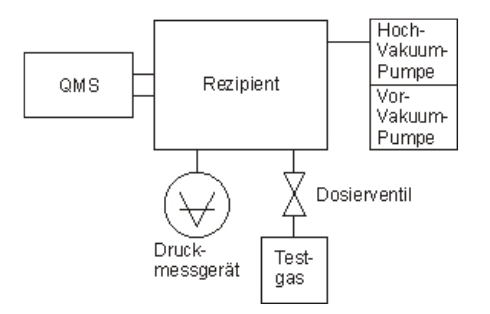
\includegraphics[scale = 0.5]{C:/Users/Marcus/Desktop/aufbau.png}
	\centering
	\caption{Aufbau des Raster-Tunnelmikroskops}
	\label{diagramm_aufspaltung}
\end{figure}

\section{	Durchführung}

Bevor Messungen am Versuchsaufbau durchgeführt werden können müssen die Messspitze und die zu untersuchende Graphitoberfläche präpariert werden. Dafür wurde die alte Messspitze zunächst aus dem Aufbau entfernt und mit einer Zange so abgekniffen, das eine möglichst dünne Spitze erzeugt wurde. Des Weiteren wurde mit einer Lage Tesafilm die oberste Schicht der Graphitprobe entfernt, um mögliche Verunreinigungen zu entfernen. Anschließend haben wir die Spitze wieder in den Messkopf eingesetzt und mittels einer Mikrometerschraube per Hand an die Probe angenähert. Mit Hilfe eines Schrittmotors wurde die Spitze dann bis auf wenige $\AA$ angenähert, bis ein vorher festgelegter Tunnelstrom messbar war. Danach wurde der Motor abgenommen und die Schutzglocke aufgesetzt. Danach haben wir verschiedene Messungen mit Variationen der Parameter, wie z.B. der angelegten Bias Spannung (zwischen Probe und Spitze) oder des festgelegten Tunnelstroms gemacht, um möglichst gute Aufnahmen der Graphit-Oberfläche zu bekommen. Atomare Auflösung konnten wir dabei allerdings nicht erreichen.

\end{document}